\documentclass[11pt]{article}

\input{../utils/preamble_problemas}
\usetikzlibrary{decorations.pathmorphing}

\title{Cálculo avanzado}
\author{Dpto. de Ingenería Mecánica}


\begin{document}
% \maketitle

\begin{center}
	\framebox[1.0\textwidth][c]{
		\huge{\textsc{Cálculo Avanzado}}
	}
\end{center}

\begin{center}
	\vspace{\baselineskip}
	\Large{\textsc{Departamento de Ingenería Mecánica}} \\
	\textsc{Facultad Regional La Plata} \\
	\textsc{Universidad Tecnológica Nacional}
\end{center}

% \vspace{1em}

\begin{center}
	\begin{tabular}{r l}
		\textbf{Práctica:}            & Unidad 7.                   \\
		\textbf{Tema:}                & Autovalores y autovectores. \\
		\textbf{Profesor Titular:}    & Manuel Carlevaro.           \\
		\textbf{Ayudante de Primera:} & Christian Molina.           \\
	\end{tabular}\end{center}

\vspace{1em}
\begin{question}
	Compruebe que
	\[ \bm{v} = \begin{bmatrix} 7 \\ 5 \end{bmatrix} \]
	es un autovector de
	\[ \bm{A} =
		\begin{bmatrix}
			53 & -70 \\
			35 & -46
		\end{bmatrix} \]
	¿Cuál es el autovalor asociado?
\end{question}

\begin{question} % Problemas resueltos Murcia p.4 pg 36

	Para la matriz cuadrada $\bm{A}$:
	\[ \bm{A} = \begin{bmatrix} 179 & -99  \\
		                255 & -139\end{bmatrix} \]
	el vector $\bm{v} = [3, 5]^{\intercal}$ es un autovector. Compruebe esta afirmación y determine el autovalor asociado.
\end{question}

\begin{question} % Problemas resueltos Murcia p.3 pg 36
	Si $\bm{u}$ y $\bm{v}$ son dos autovectores de la matriz cuadrada $\bm{A}$, ambos asociados al autovalor $\lambda$:
	\begin{enumerate}[a)]
		\item ¿Es $\bm{u} + \bm{v}$ un autovector de $\bm{A}$?. En caso afirmativo, ¿cuál es su autovector?
		\item ¿Es $\bm{v}$ un autovector de la matriz $3 \bm{A}$?. En caso afirmativo, ¿cuál es el autovalor asociado?
	\end{enumerate}
\end{question}

\begin{question} % Quarteroni 5.13 ej. 2 pg. 258
	Utilizando los círculos de Gerschgorin, localice el espectro de la matriz
	\[ \bm{A} =
		\begin{bmatrix}
			1  & 2 & -1 \\
			2  & 7 & 0  \\
			-1 & 0 & 5
		\end{bmatrix} \]
\end{question}

\begin{question} % Problemas resueltos Murcia p.22 pg 42
	Halle los autovalores y autovectores de la matriz
	\[ \bm{A} = \begin{bmatrix} -13 & 20 \\ -12 & 18 \end{bmatrix} \]
\end{question}


\begin{question} % Problemas resueltos Murcia p.25 pg 43
	Halle los autovalores y autovectores de la matriz
	\[ \bm{A} = \begin{bmatrix} 2 & 0 & 0 \\ 1 & 0 & 1 \\ 0 & 0 & 2 \end{bmatrix} \]
\end{question}

\begin{question}
	Utilice el método de las potencias para determinar el autovalor dominante y su autovector asociado de las matrices:
	\begin{multicols}{3}
		\begin{enumerate}[a)]
			\item
			      \[ \bm{A} = \begin{bmatrix} 4 & 2 & 3 \\ 3 & 0 & 4 \\ 1 & 2 & 5 \end{bmatrix} \]
			\item
			      \[ \bm{B} = \begin{bmatrix} 0 & 1 & 0 & 1 & 0 \\ 1 & 0 & 1 & 0 & 1 \\ 0 & 1 & 0 & 1 & 0 \\ 1 & 0 & 1 & 0 & 1 \\ 0 & 1 & 0 & 1 & 0 \end{bmatrix} \]
			\item
			      \[ \bm{C} = \begin{bmatrix}
					      1  & 2  & 3  & 4  & 5  & 6  \\
					      7  & 8  & 9  & 10 & 11 & 12 \\
					      13 & 14 & 15 & 16 & 17 & 18 \\
					      19 & 20 & 21 & 22 & 23 & 24 \\
					      25 & 26 & 27 & 28 & 29 & 30 \\
					      31 & 32 & 33 & 34 & 35 & 36
				      \end{bmatrix} \]

		\end{enumerate}
	\end{multicols}
\end{question}

\begin{question} % Burden Faires Ejemplo 3 pg. 434
	Muestre que se puede formar una base para $\mathbb{R}^3$ usando los autovalores de la matriz
	\[ \bm{A} = \begin{bmatrix} 2 & 0  & 0 \\
		                1 & 1  & 2 \\
		                1 & -1 & 4\end{bmatrix} \]
\end{question}

\begin{question} % Burden Faires Ejemplo 4 pg. 434
	Muestre que ningún conjunto de autovectores de la matriz $3 \times 3$
	\[ \bm{B} = \begin{bmatrix} 2 & 1 & 0 \\
		                0 & 2 & 0 \\
		                0 & 0 & 3\end{bmatrix} \]
	puede formar una base en $\mathbb{R}^3$.
\end{question}

\begin{question} % Burden Faires Ejemplo 5, pg 435
	\begin{enumerate}[a)]
		\item Muestre que los vectores $\bm{v}_1 = [0, 4, 2]^{\intercal}$ $\bm{v}_2 = [-5, -1, 2]^{\intercal}$ y $\bm{v}_3 = [1, -1, 2]^{\intercal}$ forman un conjunto ortogonal.
		\item Use el conjunto anterior para formar una base ortonormal.
	\end{enumerate}
\end{question}


\begin{question} % Burden Faires Ejemplo 6, pg 435
	Use el proceso de Gram-Schmidt para determinar un conjunto de vectores ortogonales a partir de los vectores linealmente independientes:
	\[ \bm{x}_1 = [1, 0, 0]^{\intercal}, \; \bm{x}_2 = [1, 1, 0]^{\intercal}, \; \bm{x}_3 = [1, 1, 1]^{\intercal} \]
\end{question}

\begin{question} % Burden Faires Ejemplo 1, pg 437
	Muestre que la matriz
	\[ \bm{Q} = [\bm{u}_1, \bm{u}_2, \bm{u}_3] =
		\begin{bmatrix} 0                    & -\frac{\sqrt{30}}{6}  & \frac{\sqrt{6}}{6}  \\[0.3em]
		                \frac{2 \sqrt{5}}{5} & -\frac{\sqrt{30}}{30} & -\frac{\sqrt{6}}{6} \\[0.3em]
		                \frac{\sqrt{5}}{5}   & \frac{\sqrt{30}}{15}  & \frac{\sqrt{6}}{3}\end{bmatrix} \]
	formada a partir del conjunto ortonormal de vectores encontrado en el problema 3, es una matriz ortogonal.
\end{question}

\begin{question}
	Considere el sistema mecánico de la Figura \ref{fig:sistema}, compuesto por tres masas
	deslizantes sobre una superficie horizontal sin fricción, acopladas mediante resortes
	lineales y ancladas a paredes fijas en los extremos.

	\begin{figure}[h]
		% \centering
		% \begin{tikzpicture}[scale=0.8, thick]
		% 	% Bases fijas
		% 	\draw[gray, thick] (0.0,0.75) -- (0.0,-0.75);
		% 	\draw[gray, thick] (6.5,0.75) -- (6.5,-0.75);
		%
		% 	% Resortes
		% 	\foreach \i in {0,2,4} {
		% 			\draw[decorate,decoration={aspect=0.3, segment length=2mm, amplitude=2mm,coil}]
		% 			(\i,0) -- (\i+1,0);
		% 		}
		% 	\draw[decorate,decoration={aspect=0.3, segment length=2mm, amplitude=2mm,coil}]
		% 	(6,0) -- (6.5,0);
		%
		% 	% Masas
		% 	\foreach \i/\label in {1/1, 3/2, 5/3} {
		% 			\draw[fill=blue!20] (\i,-0.5) rectangle ++(1,1);
		% 			\node at (\i+0.5,0) {\large $m_{\label}$};
		% 		}
		% \end{tikzpicture}
		% \caption{Sistema de tres grados de libertad masa-resorte.}
		% \label{fig:sistema}
		\begin{center}
			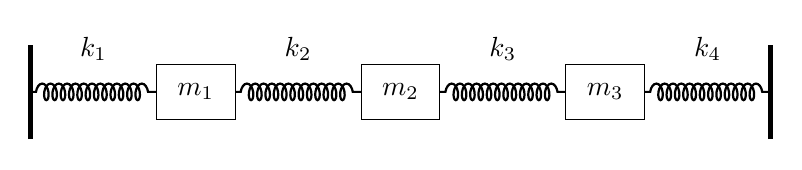
\begin{tikzpicture}[
					wall/.style={line width=2pt},
					mass/.style={draw, thick, minimum width=1.1cm, minimum height=0.85cm, fill=gray!10},
					spring/.style={decorate, decoration={coil, segment length=3pt, amplitude=3pt, pre length=2pt, post length=2pt}, thick},
					label distance/.initial=0.45cm
				]
				% Parámetros de geometría
				\def\L{1.6}      % longitud de cada resorte
				\def\w{1.0}      % ancho de cada masa
				\def\h{0.7}      % alto de cada masa
				\def\y{0}        % línea central vertical

				% --- Pared izquierda ---
				\draw[wall] (0,\y-0.6) -- (0,\y+0.6);

				% --- Resorte k1 ---
				\draw[spring] (0,\y) -- (\L,\y);
				\node at (\L/2, \y+0.55) {$k_1$};

				% --- Masa m1 ---
				\draw (\L,\y-\h/2) rectangle (\L+\w,\y+\h/2);
				\node at (\L+\w/2, \y) {$m_1$};

				% --- Resorte k2 ---
				\draw[spring] (\L+\w,\y) -- (2*\L+\w,\y);
				\node at (\L+\w+\L/2, \y+0.55) {$k_2$};

				% --- Masa m2 ---
				\draw (2*\L+\w,\y-\h/2) rectangle (2*\L+2*\w,\y+\h/2);
				\node at (2*\L+\w+\w/2, \y) {$m_2$};

				% --- Resorte k3 ---
				\draw[spring] (2*\L+2*\w,\y) -- (3*\L+2*\w,\y);
				\node at (2*\L+2*\w+\L/2, \y+0.55) {$k_3$};

				% --- Masa m3 ---
				\draw (3*\L+2*\w,\y-\h/2) rectangle (3*\L+3*\w,\y+\h/2);
				\node at (3*\L+2*\w+\w/2, \y) {$m_3$};

				% --- Resorte k4 ---
				\draw[spring] (3*\L+3*\w,\y) -- (4*\L+3*\w,\y);
				\node at (3*\L+3*\w+\L/2, \y+0.55) {$k_4$};

				% --- Pared derecha ---
				\draw[wall] (4*\L+3*\w,\y-0.6) -- (4*\L+3*\w,\y+0.6);

			\end{tikzpicture}
			\caption{Sistema de tres grados de libertad masa-resorte.}
			\label{fig:sistema}
		\end{center}
	\end{figure}


	\noindent\textbf{Datos numéricos:}
	\[
		\begin{aligned}
			m_1 & = 1.0\ \text{kg}, & \quad m_2         & = 2.0\ \text{kg}, & \quad m_3 & = 1.5\ \text{kg}, \\
			k_1 & = 20\ \text{N/m}, & \quad k_2         & = 15\ \text{N/m}, & \quad k_3 & = 10\ \text{N/m},
			    & \quad k_4         & = 25\ \text{N/m}.
		\end{aligned}
	\]

	Sean $x_1(t)$, $x_2(t)$ y $x_3(t)$ los desplazamientos de cada masa respecto a su
	posición de equilibrio estático.

	\noindent	\textbf{Consignas}

	\begin{enumerate}
		\item \textbf{Ecuaciones de movimiento:} aplicando la Segunda Ley de Newton,
		      obtenga el sistema de tres ecuaciones diferenciales ordinarias acopladas que gobiernan
		      el movimiento del sistema. Expréselo en forma matricial:
		      \[
			      M\ddot{\mathbf{x}}(t) + K\mathbf{x}(t) = \mathbf{0},
		      \]
		      identificando explícitamente las matrices de masa $M \in \mathbb{R}^{3\times 3}$ y
		      de rigidez $K \in \mathbb{R}^{3\times 3}$.

		\item \textbf{Problema de autovalores generalizado:} asumiendo una solución de
		      vibración libre del tipo $\mathbf{x}(t) = \mathbf{u}\,e^{i\omega t}$, demuestre que
		      el problema se reduce a:
		      \[
			      K\mathbf{u} = \omega^2 M\mathbf{u}.
		      \]
		      Identifique qué representan físicamente $\omega$ (autovalores) y $\mathbf{u}$
		      (autovectores).

		\item \textbf{Resolución numérica:} resuelva el problema de autovalores para los
		      datos dados. Determine:
		      \begin{itemize}
			      \item Las tres frecuencias naturales $\omega_n$ (rad/s) y sus periodos
			            $T_n = 2\pi/\omega_n$.
			      \item Los tres modos normales de vibración $\mathbf{u}^{(n)}$, normalizados
			            de modo que la masa generalizada sea la unidad:
			            $\mathbf{u}^{(n)T} M \mathbf{u}^{(n)} = 1$.
		      \end{itemize}

    \item \textbf{Normalización respecto de la masa:} cambie la representación por medio de la representación normalizada respecto de la masa:
      \[ \phi^{(n)} = \frac{\mathbf{u}^{(n)}}{\sqrt{\mathbf{u}^{(n)T} M \mathbf{u}^{(n)}}} \]

		\item \textbf{Interpretación física:} grafique cada modo de vibración y describa
		      cualitativamente el movimiento de las masas en cada caso (identifique modos, masas
		      que se mueven en fase o en contrafase, etc.).

		\item \textbf{Respuesta temporal:} suponga las condiciones iniciales
		      $\mathbf{x}(0) = [0.1,\ 0,\ 0]^T$ m y $\dot{\mathbf{x}}(0) = \mathbf{0}$.
		      Obtenga la solución temporal $\mathbf{x}(t)$ por superposición modal y grafique
		      $x_1(t)$, $x_2(t)$ y $x_3(t)$ para $t \in [0, 10]$ s.
	\end{enumerate}

\end{question}

\end{document}
